% 1977 年江苏南通卷第九题：正四棱锥 P-ABCD（P 顶点、O 底面中心），
% 高 PO 与底面对角线 AC 为虚线（按源卷第 5 页布局）
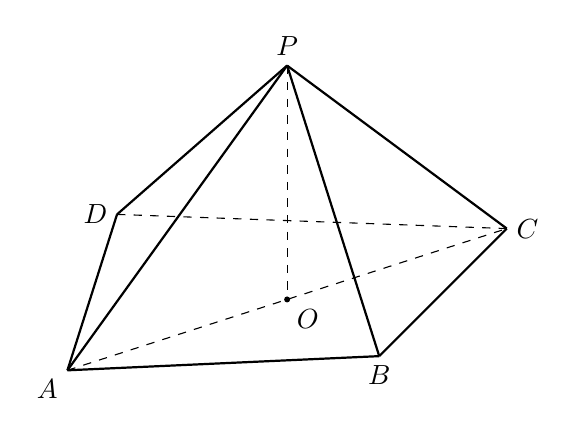
\begin{tikzpicture}[scale=0.9]
  \coordinate (A) at (0,0);
  \coordinate (B) at (4.4,0.2);
  \coordinate (C) at (6.2,2.0);
  \coordinate (D) at (0.7,2.2);
  \coordinate (P) at (3.1,4.3);
  \coordinate (O) at (3.1,1.0);
  \draw[thick] (P)--(A);
  \draw[thick] (P)--(B);
  \draw[thick] (P)--(C);
  \draw[thick] (P)--(D);
  \draw[thick] (A)--(B);
  \draw[thick] (B)--(C);
  \draw[thick] (D)--(A);
  \draw[dashed] (D)--(C);
  \draw[dashed] (A)--(C);
  \draw[dashed] (P)--(O);
  \fill (O) circle (1.2pt) node[below right] {$O$};
  \node[above] at (P) {$P$};
  \node[below left] at (A) {$A$};
  \node[below] at (B) {$B$};
  \node[right] at (C) {$C$};
  \node[left] at (D) {$D$};
\end{tikzpicture}
